% DivaPreprocessing
\chapter{Running analysis \label{chap:running}}

Once all the input files are prepared, you are ready to create analysed gridded fields. The whole procedure is described in the present chapter.

\minitoc

\section{Running a simple analysis}
%----------------------------------


\subsection{\command{divadress}}
%-----------------------------

The simplest procedure to carry out an analysis with \diva is using the command \command{divadress}, which performs the four following operations:

\begin{enumerate}
\item \command{divaclean}
\item \command{divamesh}
\item \command{divacalc}
\item \command{divaqcbis}
\end{enumerate}

\subsection{\command{divamesh}}
%-----------------------------

Generates the finite-element mesh based on contour(s) specified in file \file{coast.cont} and correlation length provided in \file{param.par}; remember that the correlation length shall have an appropriate value in order to obtain a correct mesh:
\begin{itemize}
\item Contour segments should not be much smaller than finite element length; if your contour is too fine, the tool \command{divacck} can be used in order to reduce the contour resolution.
\item The typical length of a finite element should be smaller than the correlation length, otherwise the grid would be too coarse compared to the signal to resolve.
\end{itemize}


\begin{figure}[htpb]
\centering
\parbox{.7\textwidth}{
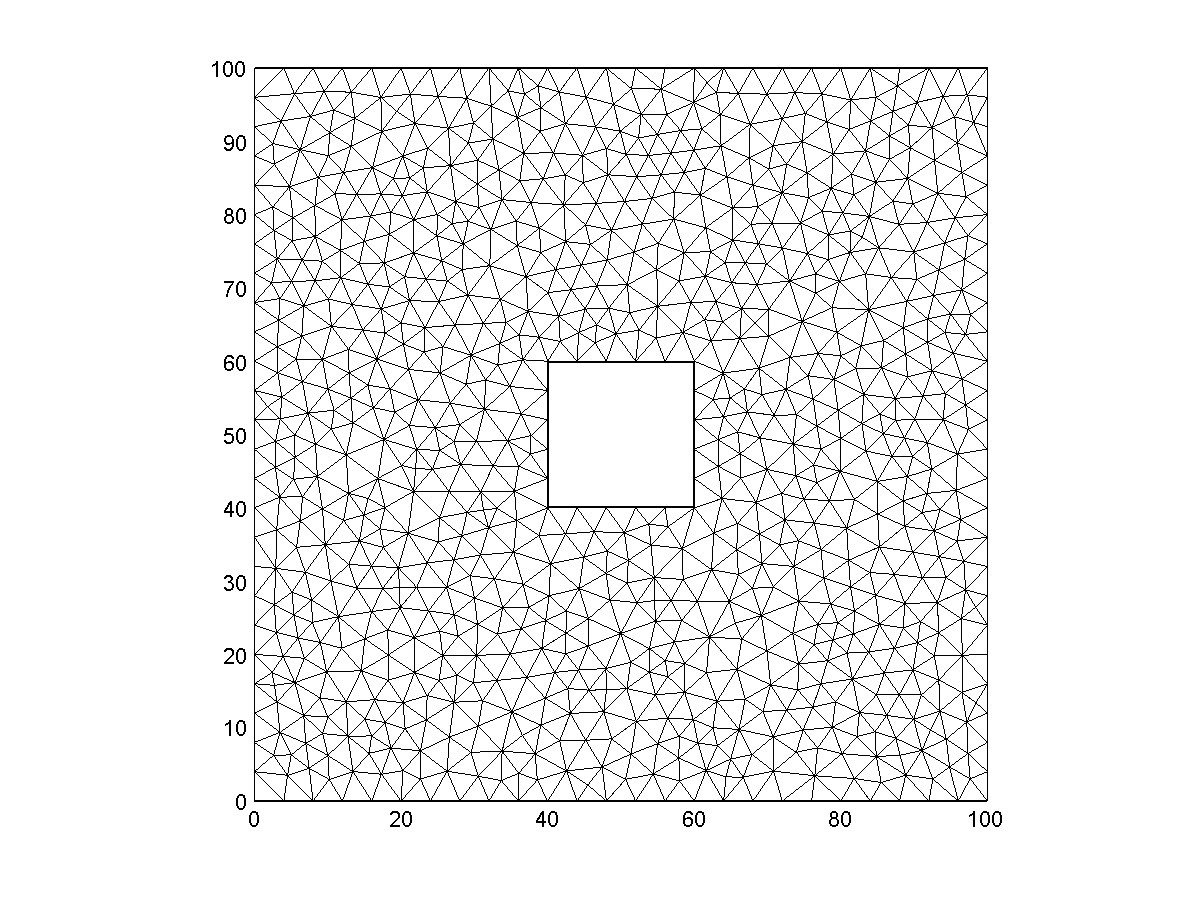
\includegraphics[width=.65\textwidth]{island_mesh}
}\parbox{.3\textwidth}{
\caption{Mesh on a simple domain.}
}
\end{figure}

Note that since version \diva-\divaversion, mesh generation takes into account coordinate change (specified by \texttt{icoord}) so that meshes are uniform in the transformed domain. 


\subsubsection{Mesh with different element sizes}

You also have the possibility to create of mesh of which the size of the elements varies over the domain. To this aim, you have to create a \textit{mesh density} file that indicates what length scale has to be applied in a determined region. This file is named \file{coast.cont.dens} and has to be placed in \directory{divastripped/input/}.

We considered the simple island case, of which the contour file given by

\begin{exfile}[htpb]
\begin{footnotesize}
\begin{verbatim}
2
4
0	0
5	0
5	5
0	5
4
2	2
2	3
3	3
3 2
\end{verbatim}
\end{footnotesize}
\caption{coast.cont}
\end{exfile}

We choose a value of $2.5$ for the global mesh (specified in \file{param.par}) and define a finer mesh around the island through the following \file{coast.cont.dens} file:

\begin{exfile}[htpb]
\begin{footnotesize}
\begin{verbatim}
1
0.125 4
1 1
4 1
4 4
1 4
\end{verbatim}
\end{footnotesize}
\caption{coast.cont.dens}
\end{exfile}

which means that we want a length scale of 0.125 in the domain defined by by the four points (1 1), (4 1), (4 4), (1 4). Be sure that the domain where you want to have a finer mesh is on the left when following the contour. The mesh generated with these conditions is presented on Fig.~\ref{fig:square}.

\begin{figure}[htpb]
\centering
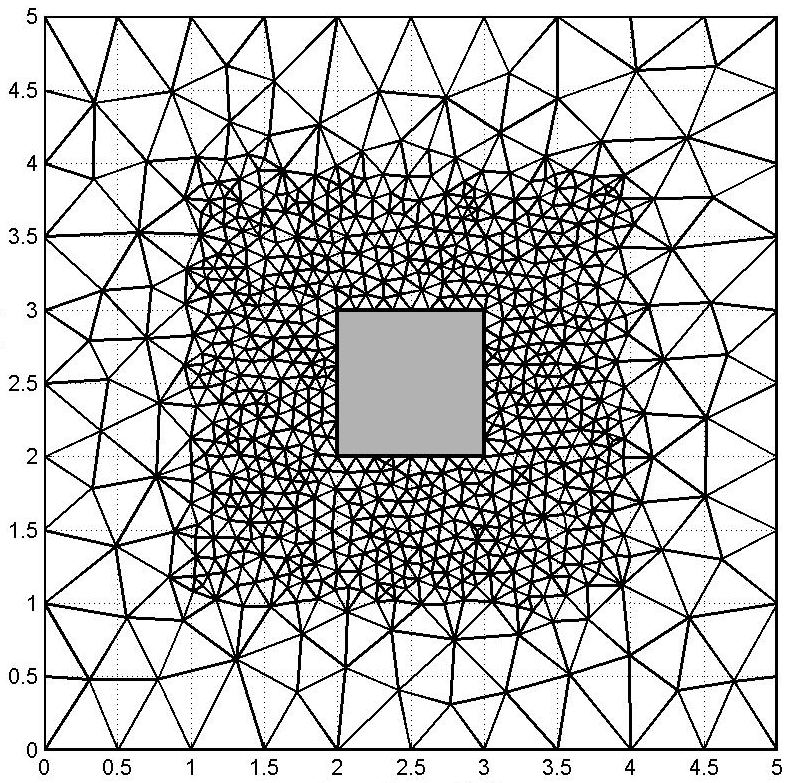
\includegraphics[width=.75\textwidth]{finer_mesh}
\caption{Mesh refinement around the island.\label{fig:square}}
\end{figure}



\subsection{\command{divacalc}\label{sec:divacalc}}
%-----------------------------

\command{divacalc} is the script that runs the analysis by solving the variational principle over the domain of interest. To work properly, it needs a data file, a parameter file, and a finite-element mesh.

\btips
As the mesh generation is often the most time-consuming part of a \diva execution, remember that once you have created the mesh, you do need to run \command{divadress} each time you want a new analysis, but just \command{divacalc}.
\etips

\begin{figure}[H]
\centering
\parbox{.7\textwidth}{
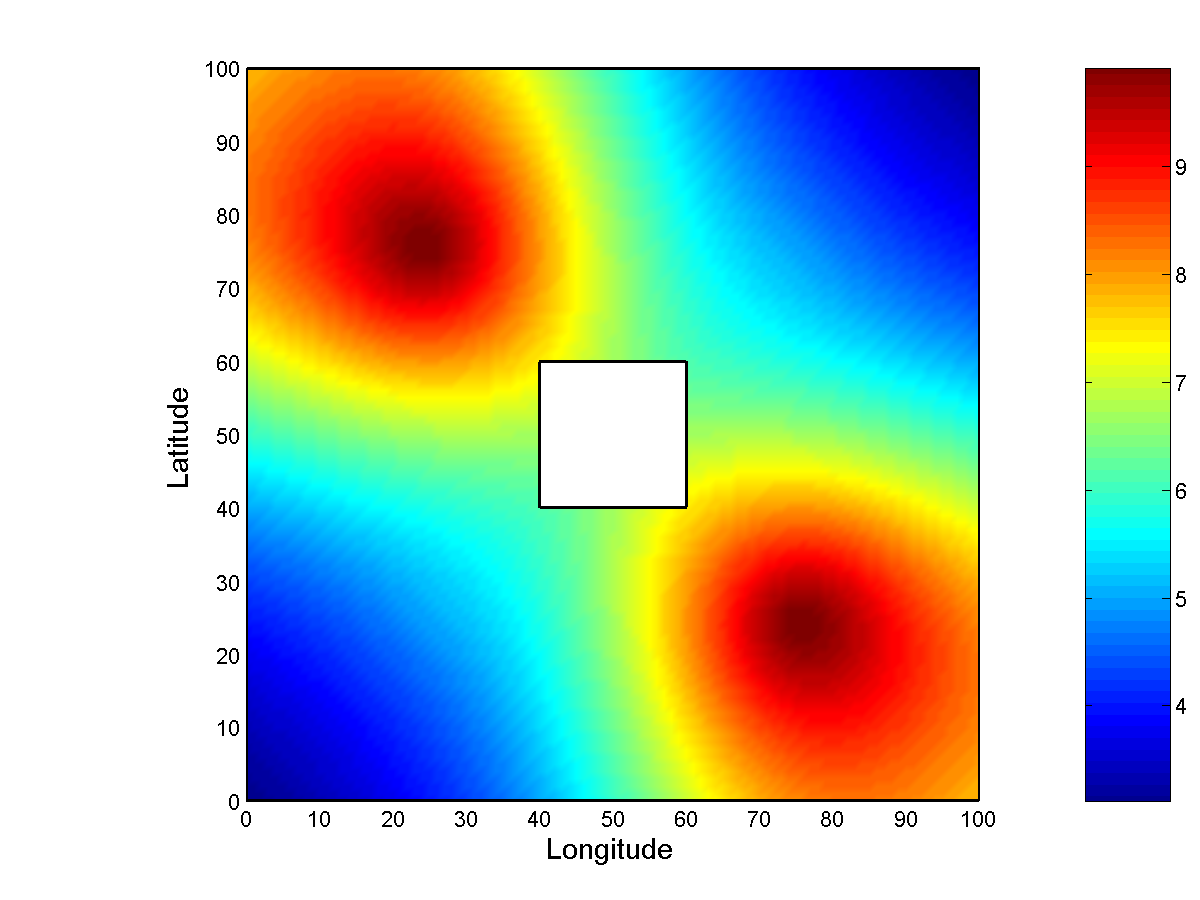
\includegraphics[width=.65\textwidth]{island_analysis}
}\parbox{.3\textwidth}{
\caption{Example of analysed field.}
}
\end{figure}


\subsubsection{Output files}
% -------------------------

\begin{itemize}
\item \file{fieldgher.anl} and \file{errorfieldgher.anl} are respectively the analysis and the error fields (in \texttt{gher} format) on the regular grid specified in \file{param.par};
\item \file{fieldascii.anl} and \file{errorfieldascii.anl} are the same as \file{fieldgher.anl} and \file{errorfieldgher.anl}, but in \texttt{ascii} format;
\item \file{valatxyascii.anl} and \file{erroratxyascii.anl} give respectively the values of the analysis and the error fields at the points specified in file \file{valatxy.coord};
\item \file{fieldatdatapoint.anl} and \file{erroratdatapoint.anl} are respectively the analysis and error fields computed at the data points (\textit{i.e.} the points from \file{data.dat});
\item \file{results.nc} (located in \directory{./output/ghertonetcdf}) is a NetCDF file containing the gridded analysis and error fields (provided error calculation is switched on).
\end{itemize}


\section{Quality control of data}
%--------------------------------

According to theoretical developments of Chapter~\ref{chap:analysisparameters}, quality control with \diva can be performed using to one of the three criteria \eqref{eq:qc1}, \eqref{eq:qc2} or \eqref{eq:qc3}, respectively implemented in \diva with \command{diva\-qc}, \command{diva\-qc\-bis} and \command{diva\-qc\-ter}. 



\subsection{Tools}

There are three tools to perform QC:
\begin{description}
\item[\command{divaqc}:] it is the most expensive version of QC, since $A_{ii}$ must be evaluated by analysis of vectors with zeros everywhere, except at the $i^{th}$ position.
\item[\command{divaqcbis}:] this version of the QC is quicker, as we replace $A_{ii}$ by its average $\frac{1}{N}\trace{\matr{A}}$.
\item[\command{divaqcter}:] the last criterion implemented is based on the RMS value of the misfit and the generalized cross validator $\Theta$. 
\end{description}

\subsection{Output files}

The corresponding outputs are given in \file{out\-liers.dat}, \file{out\-liers\-bis.dat} and \file{out\-liers\-ter.dat}.
The modules \command{divaqc*} also generate \file{outliers*.normalized.dat}, which contain, in a sorted way (from the most suspect data to less suspect), the possible outliers from the normalized misfits test \eqref{eq:qc4}.

\btips
By default, the criterion used in \command{divadress} is \command{divaqcbis}, but you can change it by editing the file \command{divadress} and replacing \command{divaqcbis} by one of the other quality test (\command{divaqc} or \command{divaqcter}).
\etips


\section{Running a semi-normed analysis}
%---------------------------------------

A semi-normed analysis consists of four steps:
\begin{enumerate}
\item create a so-called \textit{reference field}, which will act as background field (Section~\ref{sec:gridding});
\item subtract the reference field from the data values in order to work with anomalies;
\item perform an analysis on the anomalies;
\item reconstruct the field by adding the analysed anomaly field to the background (reference) field.
\end{enumerate}

These four steps are executed by running script \command{divaseminorm} and the implemented tools described hereinafter. Note that the parameters written in the original \file{param.par} file will be used during the analysis on the anomalies. Thus it is advised to specify \texttt{ireg}=0, so that no background field will be subtracted from the anomaly. 

\subsection{\command{divarefe}}
%-----------------------------

This script performs an analysis on your original data, but modify the analysis parameters: $L$ is multiplied by $5$ and $\snr$ by $0.1$. 

\subsubsection{Output files}
%---------------------------

They are the same as those created through an execution of \command{divacalc}, but assigned with a suffix \file{.ref}:
\file{fieldgher.anl.ref}, \file{fieldascii.anl.ref}, \file{valatxyascii.anl.ref} and \file{fieldatdatapoint.anl.ref}.


\subsection{\command{divaanom}}
%-----------------------------

The script use file \file{fieldatdatapoint.anl.ref} to compute the difference between data and analysed (reference) field to obtain anomalies.

\subsubsection{Output files}
%---------------------------

File \file{data.dat} contains anomalies instead of the original data, while file \file{data.dat.full} is the copy of your original data file.


\subsection{\command{divacalc}}
%-----------------------------

This command was previously described (Section~\ref{sec:divacalc}). The only difference is that it is applied here on anomalies.


\subsection{\command{divasumup}}
%-----------------------------

\command{divasumup} performs the last step of a semi-normed analysis: the sum of background field and analysed anomaly field. 

\subsubsection{Output files}
%---------------------------

They are the same as those created through an execution of \command{divacalc}. Note that after an execution of \command{divasumup}, \file{data.dat} contains the original data, while \file{data.dat.anom} contains the previously computed anomalies. 



\section{Extras}
%---------------

\subsection{Saving outputs}
%--------------------------

\command{divasave} is designed for saving the outputs in the folder \directory{output} to the chosen directory.

\example
\begin{lstlisting}[style=Bash]
[charles@gher13 divastripped] divasave ~/DIVA/test/
\end{lstlisting}
will save the files into \directory{\~{}/DIVA/test/}

\subsection{Checking of installation}
%------------------------------------

\command{divacheck} makes the comparison of analysis results with reference analysis (for
installation check, compiler option testing or checking of new versions)

%-------------------------------------------------------------------------------------------


\section{Analysis with advection constraint activated}
%---------------------------------------------------

The input files needed for such analysis are the same as for a basic analysis, except that you need to provide a velocity (or pseudo-velocity) field, specified through the following files:
\begin{itemize}
\item \file{Uvel.dat} and \file{Vvel.dat}, which contain the two components of the velocity. They have the same format (binary) as \file{fieldgher.anl}. An example of generation of such files is in the test case {\tt advectiontest}.
\item \file{UVinfo.dat}, which specifies the grid on which the velocity field is defined. It has the same format as \file{GridInfo.dat} or \file{TopoInfo.dat}).
\item \file{constraint.dat}, which activates the advection constraint and contains parameters $\theta$ and $\mathcal{A}$. Refer to Chapter~\ref{chap:advection} for theoretical details.
\end{itemize}

\begin{exfile}[htpb]
\begin{footnotesize}
\texttt{
-3.\\
-3.\\
0.100000001\\
0.100000001\\
61\\
61
} 
\end{footnotesize}
\caption{UVinfo.dat\label{ex:UVinfo.dat}}
\end{exfile}


\begin{exfile}[htpb]
\begin{footnotesize}
\texttt{
100 0.0
} 
\end{footnotesize}
\caption{constraint.dat\label{ex:constraint.dat}}
\end{exfile}

%Instead of reading in nodal properties, directly read in a gridded field 
%for $u,v$.
%Example on coordinate change effect
%In other words, (yes for velocity, but check for diffusion}, formulation 
%is done in cartesian coordinates (or any other unchanged coordinates). 
%For convenience \texttt{icoord=1} transforms input data (data location 
%and contour location) into cartesian grid, but diffusion coefficient 
%must be taken care of (if data in degrees and \texttt{icoord=1}, must be provided 
%in $m^2/s$ when velocities are in $m/s$)

%\paragraph{Files manupilated by advection constraint:}

% or matlab file {\tt } (TO BE created).


\subsection{Interplay with coordinate change on}
%--------------------------------------------------

In this example, we work on a region $[-1,1]\, \times\, [59,61]$ with $L=0.2$ and $\lambda=1$.
 

With no coordinate change (i.e., \texttt{icoordchange=0} in \file{param.par}), coordinates are taken as such and
a single point in the center leads to an analysis that is circular when axes on $x$ and $y$ are drawn with equal scales (Fig.~\ref{fig:nocoord}).

\begin{figure}[H]
\centering
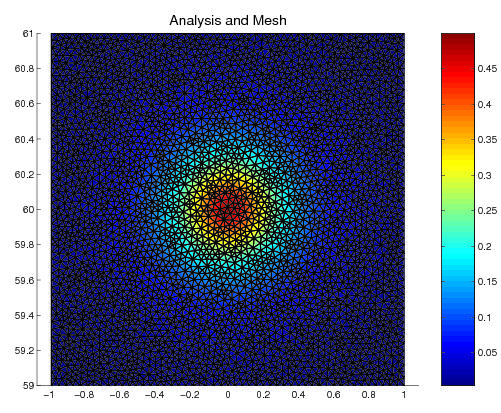
\includegraphics[width=.75\textwidth]{nocoord}
\caption{Analysis without coordinate change.\label{fig:nocoord}}
\end{figure}


On the other hand, if coordinate change is \textsl{on} (i.e., \texttt{icoordchange=1} in \file{param.par}), the analysis is isotropic in the real space.

At $60^{\circ}$ North, a degree E-W covers half the real distance of a degree S-N. On a graph scaled so that $x$ and $y$ are distances, the analysis is again isotropic (this is the desired effect). If you plot the same analysis with $x$ and $y$ axes equally spaced in degrees (as for the previous case), you will obviously get an ellipse (Fig.~\ref{fig:coord}, left).

\begin{figure}[H]
\centering
\begin{tabular}{cc}
\raisebox{.2\textwidth}{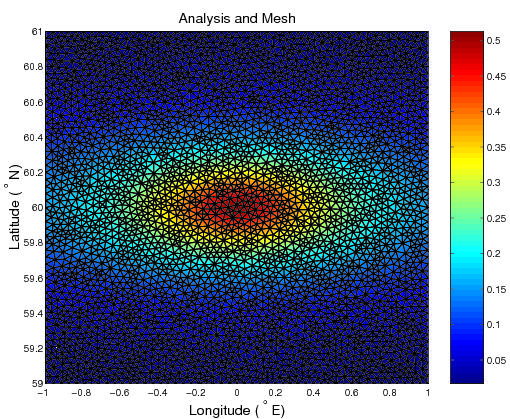
\includegraphics[width=.4\textwidth]{coord}}& 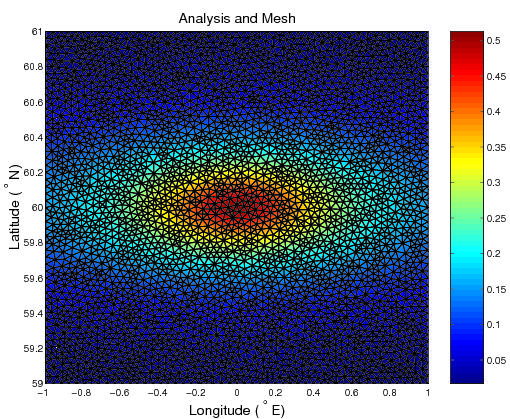
\includegraphics[width=.4\textwidth,height=.8\textwidth]{coord}\\
\end{tabular}
\caption[Analysis with coordinate change.]{Analysis with coordinate change: the two figures represent the same field, but are drawn with different scales for the axes.\label{fig:coord}}
\end{figure}


If we add an advection constraint characterized by $u=v=1 (m/s)$, the case with no coordinate change leads to a signal along the bisector (Fig.~\ref{fig:constrnocoord}).


\begin{figure}[H]
\centering
\parbox{.6\textwidth}{
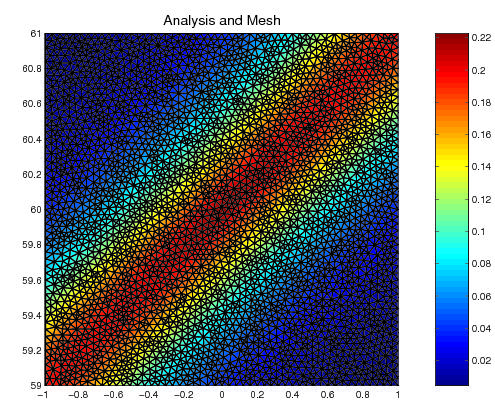
\includegraphics[width=.55\textwidth]{constrnocoord}
}\parbox{.4\textwidth}{
\caption{Analysis with advection but without coordinate change.\label{fig:constrnocoord}}
}
\end{figure}


If coordinate change is activated, the advection direction in real space is not any more along the bisector in degrees, but in km (Fig.~\ref{fig:constrdegrees}). Note that the advection constraint scales the overall velocity, so that a coordinate change does not change the intensity of the advection constraint, but only its direction.


\begin{figure}[H]
\centering
\begin{tabular}{cc}
\raisebox{.2\textwidth}{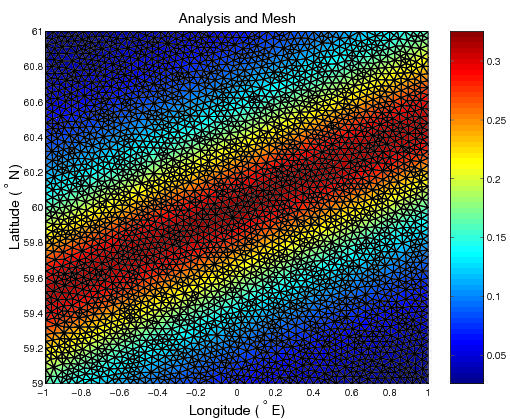
\includegraphics[width=.4\textwidth]{constrdegrees}}&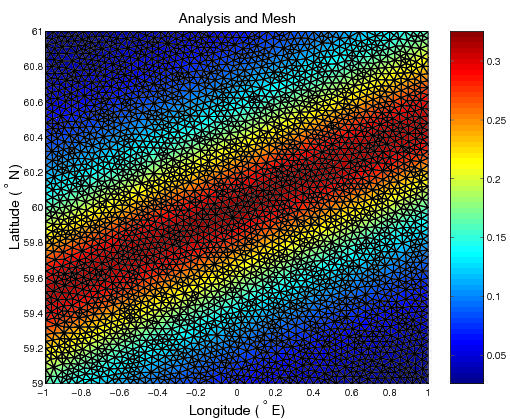
\includegraphics[width=.4\textwidth,height=.8\textwidth]{constrdegrees}
\end{tabular}
\caption{Analysis with advection and coordinate change.\label{fig:constrdegrees}}
\end{figure}




\begin{figure}[H]
\centering
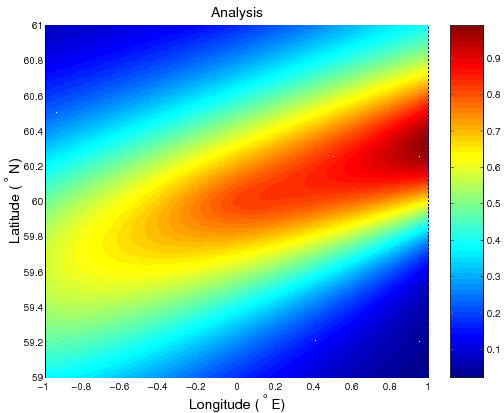
\includegraphics[width=7cm,height=14cm]{advdiffcoord}
\caption{.}
\end{figure}


Note that the diffusion coefficient is not changed. If this coefficient is given in 
Cartesian coordinates (in this case, it must be specified in $m^2/s$ if 
velocities are in $m/s$) but you provide input in degrees and do not set 
\texttt{icoord=1}, the diffusion coefficient is basically overestimated by a 
factor $10^5$.


For example, in the grid with \texttt{icoord=0} we can activate diffusion

\begin{figure}[H]
\centering
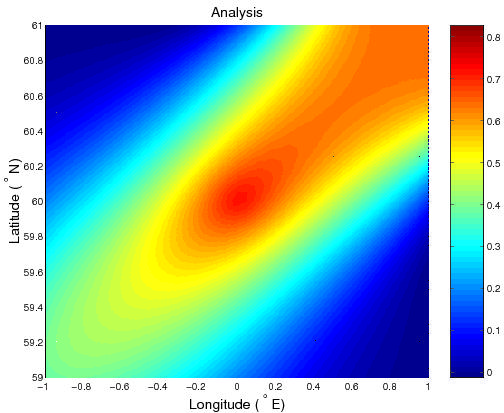
\includegraphics[width=7cm,height=14cm]{advdiffnocoord}
\caption{Diffusion coefficient divided by 110000 compared to the 
\texttt{icoord=1} case.}
\end{figure}


With no coordinate change, input values are taken as is. To recover a similar (but tilded and boundary modified) solution, we have to change manually the coefficient and divide by $110000$ (degrees to meter scaling) so that the actual Reynolds number remains the same.

%--------------------------------------------------------------------------------------------------------

\section{Summary: typical execution chains}
%------------------------------------------


\subsection{Simple analysis}
%---------------------------

It is assumed that all the input files are already prepared and the parameters correctly assigned.

\begin{enumerate}
\item \command{divaload} your\_directory
\item \command{divadress}
\item \command{divasave} your\_directory
\end{enumerate}



\subsection{Analysis with evaluation of parameters}
%--------------------------------------------------

You start with correct data and contour file, but with parameters file that needs to be adapted.

\begin{enumerate}
\item \command{divaload your\_directory}
\item \command{divafit -r} \qquad to compute the correlation length and replace its value in \file{param.par};
\item \command{divagcv -r} \qquad to compute the signal-to-noise ration and variance of the background field, and replace them in \file{param.par};
\item \command{divadress}
\item \command{divasave your\_directory}
\end{enumerate}


% to add sth